\documentclass[10pt]{beamer}

\usetheme[numbering = none, progressbar = foot]{metropolis}
\usepackage{appendixnumberbeamer}

\usepackage{graphicx}
\graphicspath{ {imagenes/} }

\usepackage[utf8]{inputenc}
\usepackage[spanish]{babel}
\usepackage{hyperref}

\usepackage{booktabs}
\usepackage[scale=2]{ccicons}


\usepackage{pgfplots}


\usepackage {tikz}
\usetikzlibrary {positioning}
\usetikzlibrary{shapes,arrows}
%\usepackage {xcolor}
\definecolor {processblue}{cmyk}{0.96,0,0,0}


\usepackage{amsmath}

\usepgfplotslibrary{dateplot}

\setbeamercolor{block title}{ fg=yellow!2, bg=black!2}

\tikzstyle{decision} = [diamond, draw, fill=green!20, 
    text width=4.5em, text badly centered, node distance=3cm, inner sep=0pt]
\tikzstyle{block} = [rectangle, draw, fill=blue!20, 
    text width=6em, text centered, minimum height=2em]
\tikzstyle{line} = [draw, -latex']
\tikzstyle{line1} = [draw, -]
\tikzstyle{cloud} = [draw, ellipse,fill=red!20, node distance=3cm,
    minimum height=2em]
\tikzstyle{place} = [draw, circle, top color =white, bottom color = processblue!20, draw,processblue , text=blue , minimum width =1.5 cm, double distance=2pt]



%\setsansfont[BoldFont={Fira Sans SemiBold}]{Fira Sans Book}
%\setsansfont[BoldFont={Fira Sans SemiBold}]{Fira Sans Book}

\usepackage{xspace}
\newcommand{\themename}{\textbf{\textsc{metropolis}}\xspace}


\title{Fluid Genetic Algorithm} 
\subtitle{Una alternativa al Algoritmo Genético Simple}
\date{\today}
\author{Semenov Flores Dimitri \\
		Perea Edgar Samuel}
\institute{Universidad Nacional Autonoma de México}
% \titlegraphic{\hfill\includegraphics[height=1.5cm]{logo.pdf}}

\begin{document}

\maketitle

\begin{frame}{Table of contents}
  \setbeamertemplate{section in toc}[sections numbered]
  \tableofcontents[hideallsubsections]
\end{frame}

\section{Introducción}

\begin{frame}{¿Qué es una metaheurística?}

	Son procesos heurísticos de una mayor abstracción que buscan resolver problemas
	para los cuales no existen algoritmos o heuríticas específicas que den \alert{soluciones
	satisfactorias}.
	
	Se busca que los métodos usados puedan \alert{escapar} de soluciones óptimas locales y que
	\alert{exploren} de forma robusta el dominio del problema.

\end{frame}

\begin{frame}{Algunos conceptos de biología}

	\begin{itemize}
		
		\item Un \alert{cromosoma} es una larga molécula de ADN (Ácido Desoxirribonucleico),
		 formada por cuatro distintos compuestos más simples llamados bases o nucleótidos
		 
		 \item Cada subcadena de tres nucleótidos codifica un aminoácido diferente que al
		unirse con los generados por otros tercetos, formará una proteína.
		
		\item Al conjunto de nucleótidos que codifican una proteína completa se
		 les llama \alert{genes}.
		 
		 \item El conjunto de todos los cromosomas, es decir, toda la información
		  genética de un individuo se llama genoma y el conjunto de
		  genes contenidos en el genoma \alert{genotipo}.
	
	\end{itemize}

\end{frame}


\begin{frame}{Ramas de Desarrollo}

	\begin{itemize}[<+- | alert@+>]
    
    	\item Adaptabilidad para la resolución de problemas en múltiples disciplinas
    	
    	\item Hibridación con otros métodos o técnicas
    	
    	\item Perfeccionamiento de los parámetro de entrada.
  
    \end{itemize}

\end{frame}

\section{El Algoritmo Genético Simple}


\begin{frame}{Algoritmo Genético Simple}

	El algoritmo genético simple (AGS) es una \alert{metaheurística} propuesta por
	John Holland en 1960 basada en los principios de selección y evolución
	propuesto por Darwin.
	
	En ella se toma una población de individuos que representan soluciones
	a un problema de optimización, estas \alert{evolucionan} de forma discreta en el tiempo
	hasta llegar a un criterio de paro.
	
	Los individuos se encuentrar codificados, usualmente de forma binaria
	
\end{frame}


\begin{frame}{Componentes del Algoritmo Genético Simple}

	\begin{itemize}[<+- | alert@+>]
    
    	\item Función de Evaluación (Fitness)
    	
    	\item Operador de Selección (Ruleta)
    	
    		%\alert<2>{This is\only<4>{ really} important}
    
    	%\item \alert<3>{This is\only<4>{ really} important}
    
    	\item Operador de Cruzamiento (Corte de un Punto)
    
    	\item Operador de Mutación
  
    \end{itemize}
    

\end{frame}

\begin{frame}{Flujo del AGS}

\begin{tikzpicture}[node distance = 3cm, auto]
    % Place nodes
    \node [block] (init) {Inicialización población};
    \node [block, below of=init, node distance=1.5cm] (eva) {Evaluación (Fiteness)};
    \node [block, right of=eva] (selec) {Seleccionamos};
    \node [block, right of=selec] (cruz) {Se cruzan los individuos};
    \node [block, below of=cruz, node distance=2.5cm] (mut) {Mutamos los descendientes};
    \node [decision, left of=mut] (paro) {Paro};
    \node [block, below of=paro, node distance=2cm] (term) {Terminación};

% Place nodes
%    \node [block] (init) {initialize model};
%    \node [cloud, left of=init] (expert) {expert};
%    \node [cloud, right of=init] (system) {system};
%    \node [block, below of=init] (identify) {identify candidate models};
 %   \node [block, below of=identify] (evaluate) {evaluate candidate models};
  %  \node [block, left of=evaluate, node distance=3cm] (update) {update model};
   % \node [decision, below of=evaluate] (decide) {is best candidate better?};
   % \node [block, below of=decide, node distance=3cm] (stop) {stop};
    % Draw edges
    %\path [line] (init) -- (identify);
%    \path [line] (identify) -- (evaluate);
 %   \path [line] (evaluate) -- (decide);
  %  \path [line] (decide) -| node [near start] {yes} (update);
   % \path [line] (update) |- (identify);
%    \path [line] (decide) -- node {no}(stop);
 %   \path [line,dashed] (expert) -- (init);
  %  \path [line,dashed] (system) -- (init);
  %  \path [line,dashed] (system) |- (evaluate);

    % Draw edges
    \path [line] (init) -- (eva);
    \path [line] (eva) -- (selec);
    \path [line] (selec) -- (cruz);
    \path [line] (cruz) -- (mut);
    \path [line] (mut) -- (paro);
    \path [line] (paro) -- node [near start] {No} (selec);
    \path [line] (paro) -- node [near start] {Si} (term);
%    \path [line] (selec) 
%    \path [line] (update) |- (identify);
%    \path [line] (decide) -- node {no}(stop);
%    \path [line,dashed] (expert) -- (init);
%    \path [line,dashed] (system) -- (init);
%    \path [line,dashed] (system) |- (evaluate);
\end{tikzpicture}



%\begin{figure}[h]
%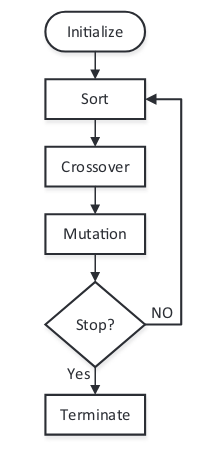
\includegraphics[width=4cm, height=7cm]{agFlow}
%\end{figure}

\end{frame}

\begin{frame}{Características a Resaltar}
  
  
  \begin{itemize}
  		\item Se maneja de forma indistinta los concpetos de cromosoma e individuo,
  			en otras palabras, tenemos que existe una relación uno a uno entre los
  			cromosomas e individuos
  			
 	\end{itemize}
 	\begin{table}
 		\caption{Cromosoma asociado al Individuo 349}
 		\begin{tabular}[t]{|c|c|c|c|c|c|c|c|c|}
			\hline
			1 & 0 & 1 & 0 & 1 & 1 & 1 & 0 & 1\\
			\hline
		\end{tabular}
 	\end{table}
\end{frame}


\section{Fluid Genetic Algorithm (FGA)}

\begin{frame}{Principal Diferencia}

	Al igual que el algoritmo genético simple es una \alert{metaheurística} basada
	en los mismos principios de la naturaleza pero con algunos conceptos nuevos 
	importantes.
	
	\begin{enumerate}
		\item No existe una relación uno a uno entre los cromosomas y los individuos,
		de hecho un cromosoma puede tener asignados múltiples individuos los cuales
		se obtendran a través de una nueva función llamada \alert{Born an Individual}
		
		\item No se utliza un operador de mutación
	\end{enumerate}



\end{frame}



\begin{frame}{Cromosomas}

	A diferencia del algoritmo genético simple los cromosomas no se manejan
	como otra representación de los individuos si no que cada cromosoma se maneja
	como la \alert{predisposición} a generar un cierto individuo.
	
	Cada una de las celdas del cromosoma representa la probabildad de que el
	individuo obtenga el valor de 1 en la celda respectiva.

	\begin{table}
 		\caption{Cromosoma para una codificación binaria}
 		\begin{tabular}[t]{|c|c|c|c|c|c|c|c|c|}
			\hline
			0.23 & 0.56 & 0.65 & 0.13 & 0.34 & 0.35 & 0.77 & 0.80 & 0.10\\
			\hline
		\end{tabular}
 	\end{table}
	

\end{frame}

\begin{frame}{Función Born an Individual}

	Relaciona los cromosomas con los individuos, dado un cromosoma genera
	un individuo de la poblacion basado en las predisposiciones del cromosoma

	\begin{table}
 		\caption{Cromosoma al aplicar Born an Individual}
 		\begin{tabular}[t]{|c|c|c|c|c|c|c|c|c|}
			\hline
			0.23 & 0.56 & 0.65 & 0.13 & 0.34 & 0.35 & 0.77 & 0.80 & 0.10\\
			\hline
			0 & 0 & 1 & 1 & 0 & 1 & 1 & 0 & 1\\
			\hline
		\end{tabular}
 	\end{table}

\end{frame}


\begin{frame}{Cálculo de Born an Individual}

	\begin{itemize}[<+- | alert@+>]
	
	\item \textbf{Generation Blue Print.} Es un cromosoma con el valor promedio
	de todos los cromosomas en una generación.
	
	\item \textbf{Global Learning Rate.} Parámetro de entrada que denominaremos
	\alert{GLR} para controlar la convergencia.
	
	\item \textbf{Local Learning Rate.} Parametro de entrada que denominaremos
	\alert{LLR} para controlar la convergencia.
	
	\item \textbf{Diversity Rate.} Parametro de entrada que denominaremos
	\alert{DR} para controlar la diversidad de la población
	
	\end{itemize}

\end{frame}

\begin{frame}{Cálculo de Born an Individual}

\begin{itemize}[<+- | alert@+>]
	\item \textbf{Blue Print Value I.} Valor de la celda I del Generation Blue
	Print al cual llamaremos \alert{BPVCi} 
	
	\item \textbf{Cromosome Value I.} Valor de la celda I del cromosoma actual
	al cual llamaremos \alert{CVCi}
	
	\item \textbf{Effective Value I.} Valor de la probabilidad con la cual se
	decidira si la celda I del individuo tomara el valor 1 o 0 al cual 
	llamaremos  \alert{EFVi}
\end{itemize}


\end{frame}

\begin{frame}{Cálculo de Born an Individual}



\begin{gather*}
	(GLR \times BPVCi + (1 - GLR) \times CVCi  < DR) \leftrightarrow  EFVi = DR\\
	(GLR \times BPVCi + (1 - GLR) \times CVCi  > (1 - DR)) \leftrightarrow EFVi = (1 - DR)\\
	Otro caso \leftrightarrow EFVi = (GLR \times BPVCi + (1 - GLR) \times CVCi
\end{gather*}



\end{frame}


\begin{frame}{Operador de Cruzamiento}

	EL proceso de cruzamiento se realiza de forma similar al algoritmo genético
	simple, con la diferencia de que se toma un parámetro extra \alert{(Local Learning Rate)}

		LLR = 0.05

		\begin{table}
 		\caption{Cromosoma A}
 		\begin{tabular}[t]{|c|c|c||c|c|c|c|}
			\hline
			0.41 & 0.26 & 0.99 & 0.21 & 0.63 & 0.39 & 0.85 \\
			\hline
			1 & 0 & 1 & 0 & 0 & 0 & 1\\
			\hline
		\end{tabular}
 	\end{table}
 	
 		\begin{table}
 		\caption{Cromosoma B}
 		\begin{tabular}[t]{|c|c|c||c|c|c|c|}
			\hline
			0.26 & 0.64 & 0.49 & 0.79 & 0.63 & 0.13 & 0.97 \\
			\hline
			0 & 1 & 1 & 1 & 1 & 0 & 0 \\
			\hline
		\end{tabular}
 	\end{table}
	
\end{frame}



\begin{frame}{Operador de Cruzamiento}

	\begin{table}
 		\caption{Descendiente}
 		\begin{tabular}[t]{|c|c|c|c|c|c|c|}
			\hline
			0.41 & 0.26 & 0.99 & 0.79 & 0.63 & 0.13 & 0.97 \\
			\hline
			1 & 0 & 1 & 1 & 1 & 0 & 0 \\
			\hline
		\end{tabular}
 	\end{table}
 	
 	\begin{table}
 		\caption{Descendiente con LLR}
 		\begin{tabular}[t]{|c|c|c|c|c|c|c|}
			\hline
			0.46 & 0.21 & 1 & 0.84 & 0.68 & 0.08 & 0.92 \\
			\hline
			1 & 0 & 1 & 1 & 1 & 0 & 0 \\
			\hline
		\end{tabular}
 	\end{table}
 	
 		\begin{table}
 		\caption{Cromosoma nuevo}
 		\begin{tabular}[t]{|c|c|c|c|c|c|c|}
			\hline
			0.46 & 0.21 & 1 & 0.84 & 0.68 & 0.08 & 0.92 \\
			\hline
		\end{tabular}
 	\end{table}

%	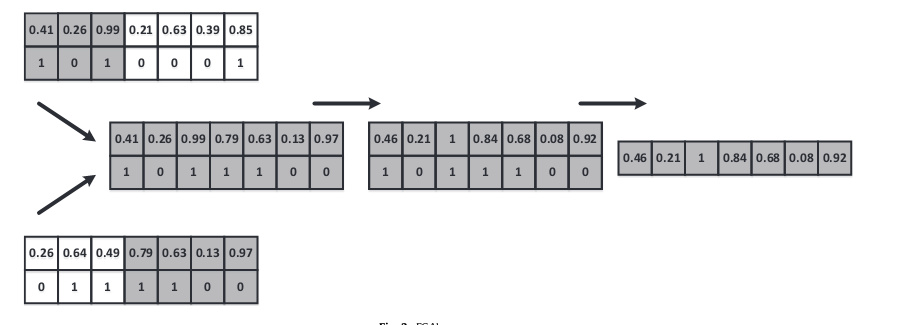
\includegraphics[width=12cm, height=6cm]{cruzamiento}

\end{frame}

\begin{frame}{Flujo FGA}

\begin{tikzpicture}[node distance = 3cm, auto]
    % Place nodes
    \node [block] (init) {Inicialización población};
    \node [block, right of=init] (born) {Born an Individual};
    \node [block, below of=born, node distance=1.5cm] (eva) {Evaluación (Fiteness)};
    \node [block, right of=eva] (selec) {Seleccionamos };
    \node [block, right of=selec] (cruz) {Se cruzan los individuos};
    \node [decision, below of=selec] (paro) {Paro};
    \node [block, below of=paro, node distance=2cm] (term) {Terminación};
    % arrows
    \path [line] (init) -- (born);
    \path [line] (born) -- (eva);
    \path [line] (eva) -- (selec);
    \path [line] (selec) -- (cruz);
    \path [line] (cruz) |- (paro);
    \path [line] (paro) -- node [near start] {No} (selec);
    \path [line] (paro) -- node [near start] {Si} (term);

\end{tikzpicture}

\end{frame}


\begin{frame}{Diferencias}

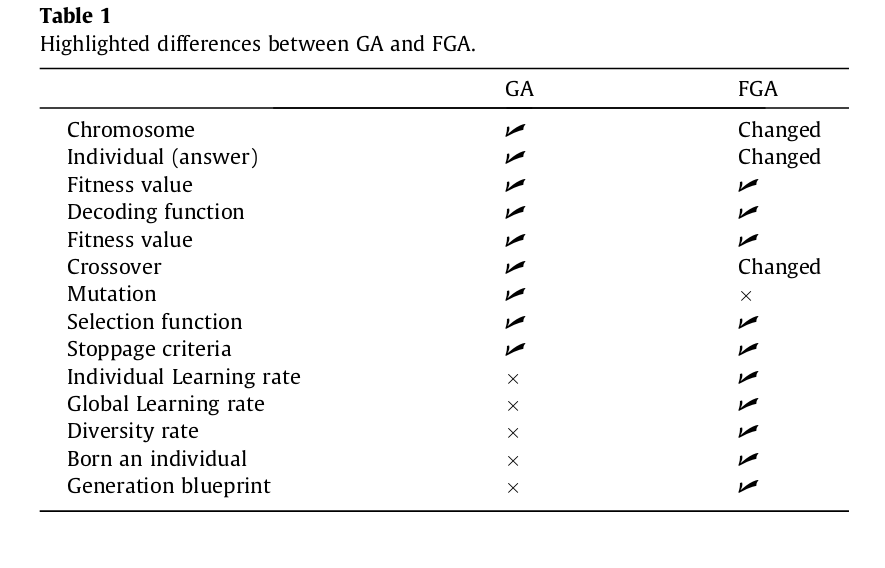
\includegraphics[width=11.5cm, height=7cm]{diferencias}

\end{frame}

\section{Experimentos y Desempeño}

\begin{frame}{Medida de Desempeño}
	
	
	Nos interesan dos puntos en el algoritmo genético:
	
	\begin{enumerate}
	
		\item El \alert{tiempo} que tarda en encontrar las soluciones óptimas al problema
		(Número de iteraciones).
		
		\item Que el algoritmo sea de confianza, esto es que genere respuestas buenas
		\alert{consistentemente} aunque tal vez no sean las mejores.
		
		
	\end{enumerate}
	
\end{frame}


\begin{frame}{Medida de Desempeño}
	\begin{itemize}[<+- | alert@+>]
    
    	\item \textbf{NESR.} Número de evaluaciones de ejecuciones
    	 exitosas.
    	
    	\item \textbf{NR.} Número de ejecuciones.
    	
    		%\alert<2>{This is\only<4>{ really} important}
    
    	%\item \alert<3>{This is\only<4>{ really} important}
    
    	\item \textbf{NSR} Número de ejecuciones exitosas.
    
    	\item \textbf{N.} Dimensión del problema.
  
    \end{itemize}
    

\end{frame}




\begin{frame}{Medida de Desempeño}
	\begin{align*}
		SP1 &= \frac{NESR \times NR}{NSR^2}\\
		SP2 &= N \times 10^4 \times (\frac{NR - NSR}{NR}) + \frac{NESR}{NSR}
	\end{align*}
\end{frame}


\begin{frame}{FGA vs AGS}

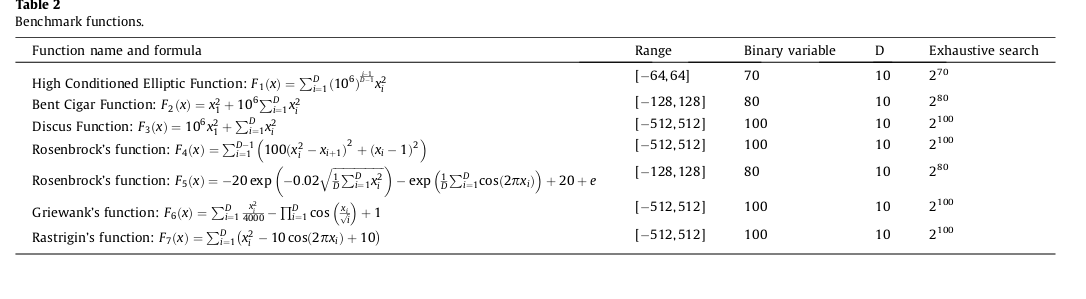
\includegraphics[width=11.5cm, height=3.5cm]{benchmarkF}

\end{frame}

\begin{frame}{FGA vs AGS}

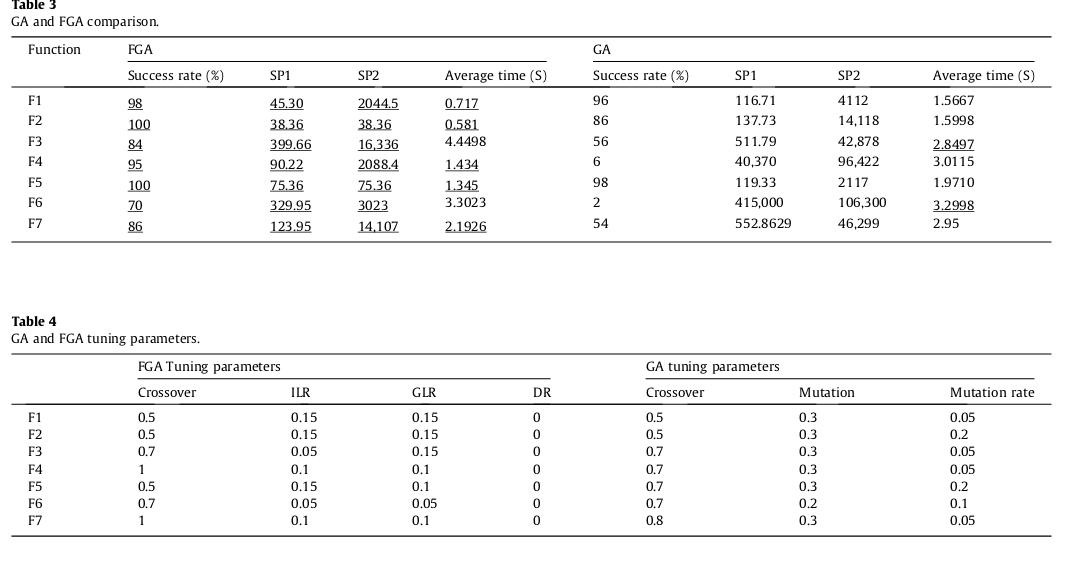
\includegraphics[width=11.5cm, height=7cm]{resultados}

\end{frame}

\begin{frame}{FGA vs AGS}

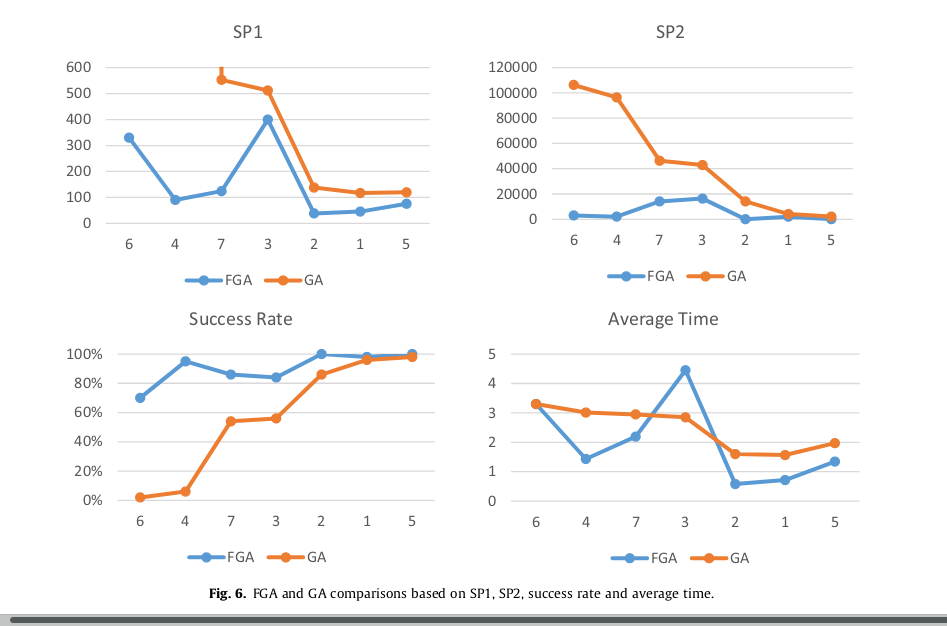
\includegraphics[width=11.5cm, height=7cm]{graphs}

\end{frame}

\section{Problema de la asignación cuadrática (QAP)}

\begin{frame}{Formulación}

	Hay un conjunto de n instalaciones y un conjutno de n localidades. Para cada
	par de localidades se tiene asignado una distancia y para cada par de instalaciones
	se tiene asignado un flujo. El problema consiste en asignar cada una de las 
	diferentes instalaciones a diferentes localidades con la meta de minimizar
	la suma de las distancias multiplicada por los flujos correspondientes.

\end{frame}

\begin{frame}{Ejemplo}

\begin{tikzpicture}[node distance = 3cm, auto]
	\node[place] (A) {$1$};
	\node[place] (B) [right = of A] {$2$};
	\node[place] (C) [right = of B] {$3$};
	\node[place] (D) [below left = of C] {$4$};
	\node[place] (E) [below right = of A] {$5$};
	
	\path [line1] (A) -- node [near start] {$50$} (B);
	\path [line1] (B) -- node [near start] {$30$} (C);
	\path [line1] (D) -- node [near start] {$40$} (B);
	\path [line1] (B) -- node [near start] {$15$} (E);
\end{tikzpicture}

\end{frame}

\begin{frame}{Modelo Matemático}
	
	\begin{itemize}
	
		\item $D_{ij}$ Distancia entre dos localidades.
		
		\item $T_{kl}$ Valor de trafico entre dos instalaciones.
		
		\item $F_{ik}$ Costo de poner la instalación k en la localidad i.
		
		\item $X_{ik}$ Función binaria que asigna 1 si y solo si la
		instalación k en la localidad i.
	
	\end{itemize}
	
	$$\sum_{i=1}^{n_{s}} \sum_{j=i}^{n_{s}} \sum_{k=1}^{n_{0}} \sum_{l=k}^{n_{0}} T_{ij}D_{kl}X_{ik}X_{jl} +
	\sum_{i=1}^{n_{s}} \sum_{k=1}^{n_{0}} F_{ik}X_{ik}= 1$$
	
\end{frame}


\begin{frame}{Cromosoma de FGA}

	Cada cromosoma tiene dos renglones de valores
	
	\begin{itemize}
	
		\item El seguno marca las instalaciones en cada celda
		
		\item  El primero marca la probabilidad de que el individuo que se genera
		 tenga la instalación indicada en el segundo renglón
	
	\end{itemize}
	

\end{frame}

\begin{frame}{Cromosoma de FGA}


	\begin{table}
 		\caption{Cromosoma para QAP (AGS)}
 		\begin{tabular}[t]{|c|c|c|c|c|}
			\hline
			4 & 1 & 3 & 5 & 2\\
			\hline
		\end{tabular}
 	\end{table}


	\begin{table}
 		\caption{Cromosoma para QAP (FGA)}
 		\begin{tabular}[t]{|c|c|c|c|c|}
			\hline
			0.1 & 0.4 & 0.6 & 0.8 & 0.3 \\
			\hline
			5 & 2 & 3 & 2 & 4\\
			\hline
		\end{tabular}
 	\end{table}


\end{frame}

\begin{frame}{Born an Individual}


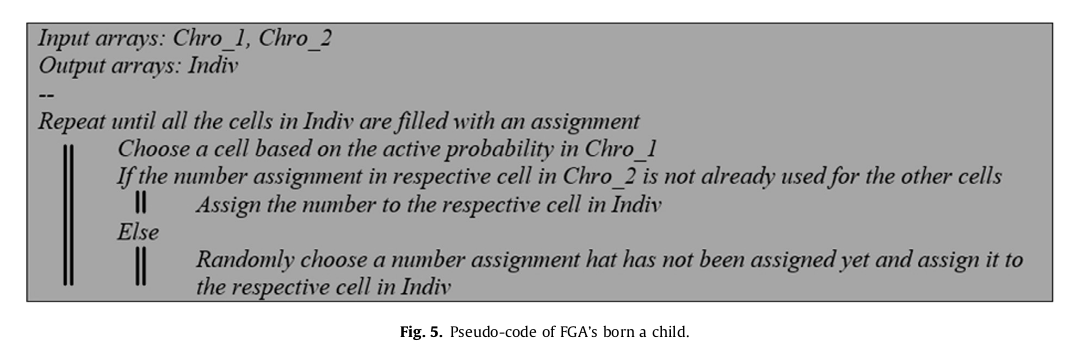
\includegraphics[width=11.5cm, height=4cm]{code}


\end{frame}

\begin{frame}{Cruzamiento}

	El cruzamiento de realiza de la misma forma pero con una diferencia clave,
	para asignar el incremento o decremento del valor LLR se realiza lo siguiente
	
	\begin{itemize}
	
		\item Si el valor de la instalación es el mismo que el de el segundo
		renglón de la respectiva celda del cromosoma, se incrementa el valor
		 de la respectiva celda en el primer renglón por el valor de LLR.
		
		\item En caso opuesto se decrementa el valor de la respectiva celda en el
		primer renglón por el valor de LLR.
	
	\end{itemize}

\end{frame}

\begin{frame}{Cruzamiento ejemplo}

	\begin{table}
 		\caption{Cromosoma A}
 		\begin{tabular}[t]{|c|c||c|c|c|}
			\hline
			0.1 & 0.4 & 0.6 & 0.8 & 0.3 \\
			\hline
			5 & 2 & 3 & 2 & 4\\
			\hline
			5 & 4 & 3 & 2 & 1\\
			\hline
		\end{tabular}
 	\end{table}
 	
 	\begin{table}
 		\caption{Cromosoma B}
 		\begin{tabular}[t]{|c|c||c|c|c|}
			\hline
			0.7 & 0.4 & 0.3 & 0.5 & 0.8 \\
			\hline
			4 & 3 & 3 & 5 & 1\\
			\hline
			4 & 2 & 5 & 3 & 1\\
			\hline
		\end{tabular}
 	\end{table}


\end{frame}

\begin{frame}{Cruzamiento ejemplo}

 	\begin{table}
 		\caption{Descendiente}
 		\begin{tabular}[t]{|c|c||c|c|c|}
			\hline
			0.1 & 0.4 & 0.3 & 0.5 & 0.8 \\
			\hline
			5 & 2  & 3 & 5 & 1\\
			\hline
			5 & 4 & 5 & 3 & 1\\
			\hline
		\end{tabular}
 	\end{table}
 	
 	 	\begin{table}
 		\caption{Descendiente con LLR}
 		\begin{tabular}[t]{|c|c||c|c|c|}
			\hline
			0.15 & 0.35 & 0.25 & 0.45 & 0.85 \\
			\hline
			5 & 2  & 3 & 5 & 1\\
			\hline
			5 & 4 & 5 & 3 & 1\\
			\hline
		\end{tabular}
 	\end{table}
 	

\end{frame}


\begin{frame}{Cruzamiento ejemplo}

 	 \begin{table}
 		\caption{Nuevo Cromosoma}
 		\begin{tabular}[t]{|c|c||c|c|c|}
			\hline
			0.15 & 0.35 & 0.25 & 0.45 & 0.85 \\
			\hline
			5 & 2  & 3 & 5 & 1\\
			\hline
		\end{tabular}
 	\end{table}
 	
\end{frame}


\begin{frame}{Pruebas}

	\begin{itemize}
	
	\item Para comparar el desempeño AGS y FGA se utilizaron 5 instancias del problema
	de la libreria \textit{QAPLIB - A Quadratic Assignment Problem Library}.
	
	\item Se utlizo una población de 100 cromosomas para AGS y 200 para FGA.
	
	\item Finalmente cada problema se realizo 10 veces por algoritmo.
	
	\end{itemize}
	
	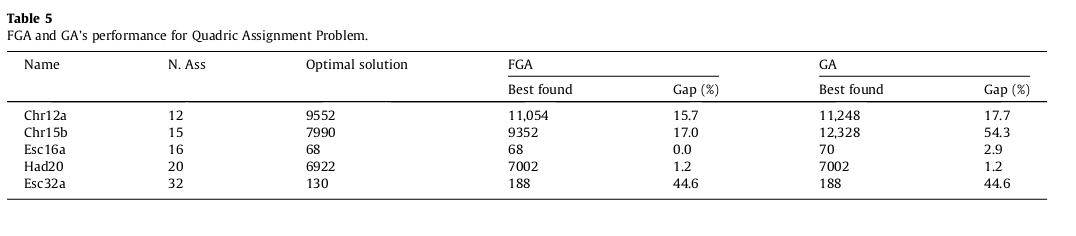
\includegraphics[width=11.5cm, height=3cm]{value}


\end{frame}


\section{Conclusiones}

\begin{frame}{Conclusiones}

	\begin{itemize}[<+- | alert@+>]
	
		\item Alto nivel de diversidad en la población.
		
		\item Cromosomas e individuos son diferentes.
		
		\item Amplio control de convergencia.
		
		\item Mayor dificultad para definir cromosomas y conservar la fluidez
		entre individuo y cromosoma.
	
	\end{itemize}

\end{frame}


\begin{frame}{Bibliografía}


\begin{thebibliography}{9}


\bibitem{PATT}
		Galaviz Jose, Kuri Ángel \emph{Algoritmos Genéticos}.
		
\bibitem{FGA}
		Ruholla Jafari-Marandi, Brian K. Smith \emph{Fluid Genetic Algorithm}.
\bibitem{VLD}
		Auger A., Hansen N \emph{Performance Evaluation of an Advanced Local Search Evolutionary Algorithm}.
%\bibitem{Metaheurística}
%		Hola mundo, \emph{bye}.
%\url{https://es.wikipedia.org/wiki/Metaheur%C3%ADstica}.
		
%\bibitem{Quadratic assignment problem}
%		\url{https://en.wikipedia.org/wiki/Quadratic_assignment_problem}.
%\bibitem{lamport94}
%\bibitem{Metaheurística}
%	\url{https://es.wikipedia.org/wiki/Metaheur%C3%ADstica}.

 % \bibitem{Quadratic assignment problem}
	%\url{https://en.wikipedia.org/wiki/Quadratic_assignment_problem}.

%	\bibitem{PATT}
%			Galaviz Jose, Kuri Ángel \emph{Algoritmos Genéticos}.
\end{thebibliography}
%		\begin{thebibliography}{5}
%		\bibitem{Metaheurística}
%		\url{https://es.wikipedia.org/wiki/Metaheur%C3%ADstica}
%
%		\bibitem{Quadratic assignment problem}
%		\url{https://en.wikipedia.org/wiki/Quadratic_assignment_problem}

%		\bibitem{PATT}
%			Galaviz Jose, Kuri Ángel \emph{Algoritmos Genéticos}.
	
%	\end{thebibliography}
%  \bibliography{Metaheurística}
%  \bibliographystyle{abbrv}

\end{frame}

\end{document}
